% Title: gl2ps_renderer figure
% Creator: GL2PS 1.4.2, (C) 1999-2020 C. Geuzaine
% For: Octave
% CreationDate: Thu Nov 11 16:28:52 2021
\setlength{\unitlength}{1pt}
\begin{picture}(0,0)
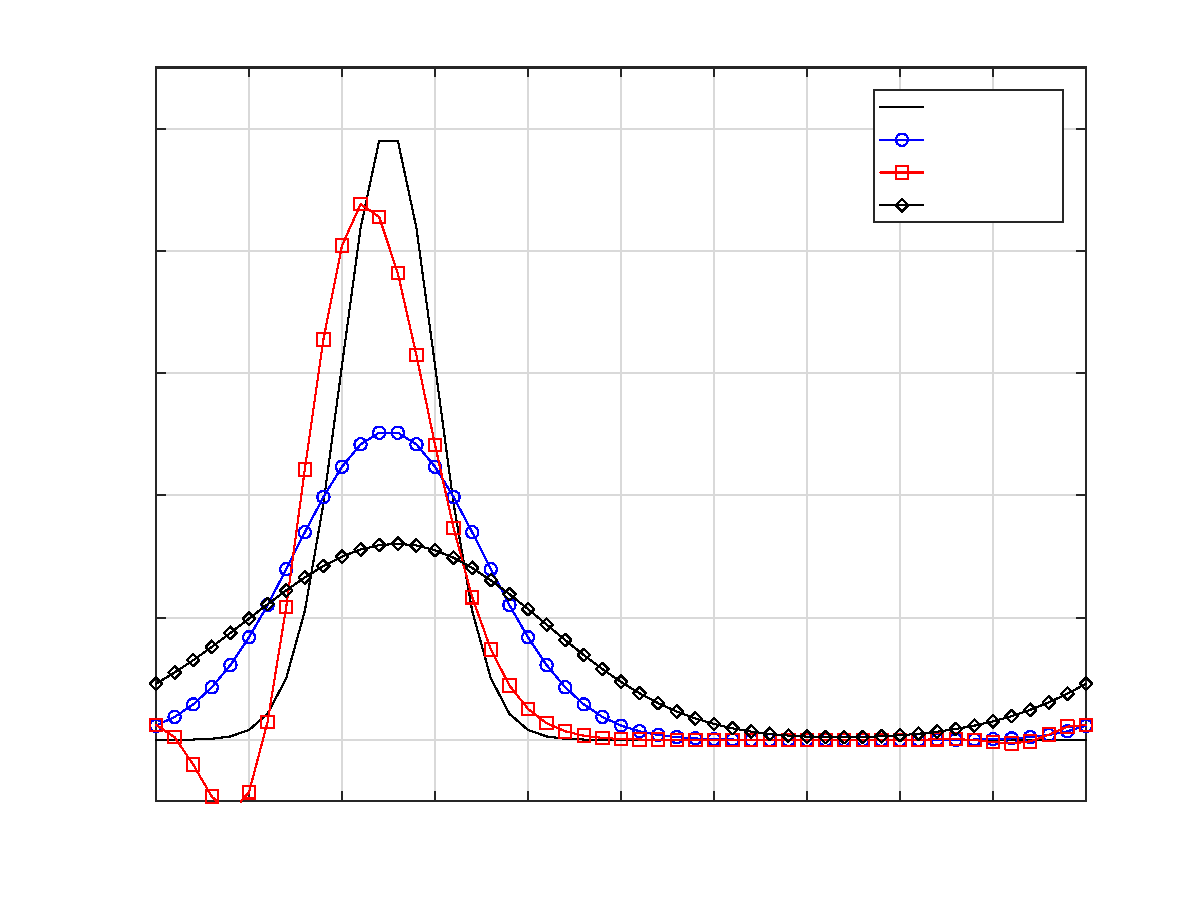
\includegraphics[scale=1]{figures/chap29/OUT2/adv0003-inc}
\end{picture}%
\begin{picture}(576,432)(0,0)
\fontsize{10}{0}\selectfont\put(74.8799,40.0181){\makebox(0,0)[t]{\textcolor[rgb]{0.15,0.15,0.15}{{0}}}}
\fontsize{10}{0}\selectfont\put(119.52,40.0181){\makebox(0,0)[t]{\textcolor[rgb]{0.15,0.15,0.15}{{0.1}}}}
\fontsize{10}{0}\selectfont\put(164.16,40.0181){\makebox(0,0)[t]{\textcolor[rgb]{0.15,0.15,0.15}{{0.2}}}}
\fontsize{10}{0}\selectfont\put(208.8,40.0181){\makebox(0,0)[t]{\textcolor[rgb]{0.15,0.15,0.15}{{0.3}}}}
\fontsize{10}{0}\selectfont\put(253.44,40.0181){\makebox(0,0)[t]{\textcolor[rgb]{0.15,0.15,0.15}{{0.4}}}}
\fontsize{10}{0}\selectfont\put(298.08,40.0181){\makebox(0,0)[t]{\textcolor[rgb]{0.15,0.15,0.15}{{0.5}}}}
\fontsize{10}{0}\selectfont\put(342.72,40.0181){\makebox(0,0)[t]{\textcolor[rgb]{0.15,0.15,0.15}{{0.6}}}}
\fontsize{10}{0}\selectfont\put(387.36,40.0181){\makebox(0,0)[t]{\textcolor[rgb]{0.15,0.15,0.15}{{0.7}}}}
\fontsize{10}{0}\selectfont\put(432,40.0181){\makebox(0,0)[t]{\textcolor[rgb]{0.15,0.15,0.15}{{0.8}}}}
\fontsize{10}{0}\selectfont\put(476.64,40.0181){\makebox(0,0)[t]{\textcolor[rgb]{0.15,0.15,0.15}{{0.9}}}}
\fontsize{10}{0}\selectfont\put(521.28,40.0181){\makebox(0,0)[t]{\textcolor[rgb]{0.15,0.15,0.15}{{1}}}}
\fontsize{10}{0}\selectfont\put(69.8755,76.8599){\makebox(0,0)[r]{\textcolor[rgb]{0.15,0.15,0.15}{{0}}}}
\fontsize{10}{0}\selectfont\put(69.8755,135.54){\makebox(0,0)[r]{\textcolor[rgb]{0.15,0.15,0.15}{{0.2}}}}
\fontsize{10}{0}\selectfont\put(69.8755,194.22){\makebox(0,0)[r]{\textcolor[rgb]{0.15,0.15,0.15}{{0.4}}}}
\fontsize{10}{0}\selectfont\put(69.8755,252.9){\makebox(0,0)[r]{\textcolor[rgb]{0.15,0.15,0.15}{{0.6}}}}
\fontsize{10}{0}\selectfont\put(69.8755,311.58){\makebox(0,0)[r]{\textcolor[rgb]{0.15,0.15,0.15}{{0.8}}}}
\fontsize{10}{0}\selectfont\put(69.8755,370.26){\makebox(0,0)[r]{\textcolor[rgb]{0.15,0.15,0.15}{{1}}}}
\fontsize{11}{0}\selectfont\put(298.08,27.0181){\makebox(0,0)[t]{\textcolor[rgb]{0.15,0.15,0.15}{{$x$}}}}
\fontsize{11}{0}\selectfont\put(49.8755,223.56){\rotatebox{90}{\makebox(0,0)[b]{\textcolor[rgb]{0.15,0.15,0.15}{{exact and approximate solutions}}}}}
\fontsize{11}{0}\selectfont\put(298.08,409.6){\makebox(0,0)[b]{\textcolor[rgb]{0,0,0}{{Finite Difference Approximations at $T$ = 0.75, $h$ = 0.02, and $\tau$ =0.01}}}}
\fontsize{9}{0}\selectfont\put(446.421,380.742){\makebox(0,0)[l]{\textcolor[rgb]{0,0,0}{{Exact}}}}
\fontsize{9}{0}\selectfont\put(446.421,364.97){\makebox(0,0)[l]{\textcolor[rgb]{0,0,0}{{Upwind}}}}
\fontsize{9}{0}\selectfont\put(446.421,349.198){\makebox(0,0)[l]{\textcolor[rgb]{0,0,0}{{Lax--Wendroff}}}}
\fontsize{9}{0}\selectfont\put(446.421,333.426){\makebox(0,0)[l]{\textcolor[rgb]{0,0,0}{{Lax--Friedrichs}}}}
\end{picture}
